\section{Test computer specifications}
\label{sec:specs}
In this section we put the relevant parts of the specifications of the
computer that was used for testing and benchmarking.

\paragraph{Software versions}

\begin{description}
\item[Operating system] Ubuntu 10.10 - the Maverick Meerkat
\item[\texttt{gcc}] (Ubuntu/Linaro 4.4.4-14ubuntu5) 4.4.5
\item[\texttt{perl}] 5.10.1 (*) built for i686-linux-gnu-thread-multi
\item[\texttt{tcl}] 8.4.16-2
\item[\texttt{re2}] Version present in the repository at the date of
  fetching: 2. March 2011.
\item[\texttt{g++}] Ubuntu/Linaro 4.4.4-14ubuntu5) 4.4.5
\end{description}


\paragraph{Technical specifications}
\begin{description}
\item[CPU] Intel(R) Core(TM) i3 CPU       M 330  @ 2.13GHz
\item[Memory] 1938 MB
\item[Storage] Samsung HM250HI
\end{description}



\section{Huffman trees}

\begin{figure}
  \centering 
  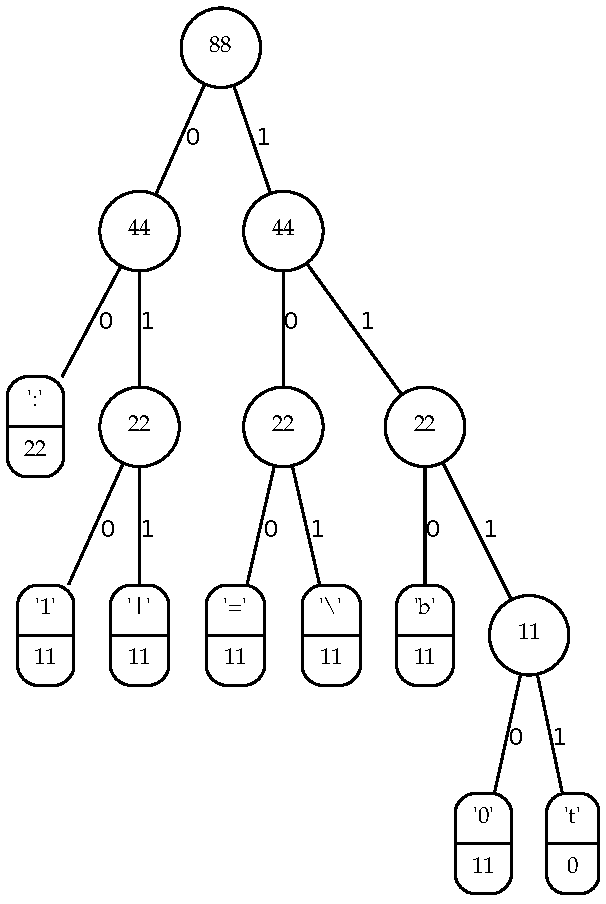
\includegraphics{optimizations/huffman2.pdf}
  \caption{Huffman tree for frequencies in table
    \ref{tab:huffman_freq}, \textsf{.*}}
  \label{fig:huffman1}
\end{figure}

\begin{figure}
  \centering
  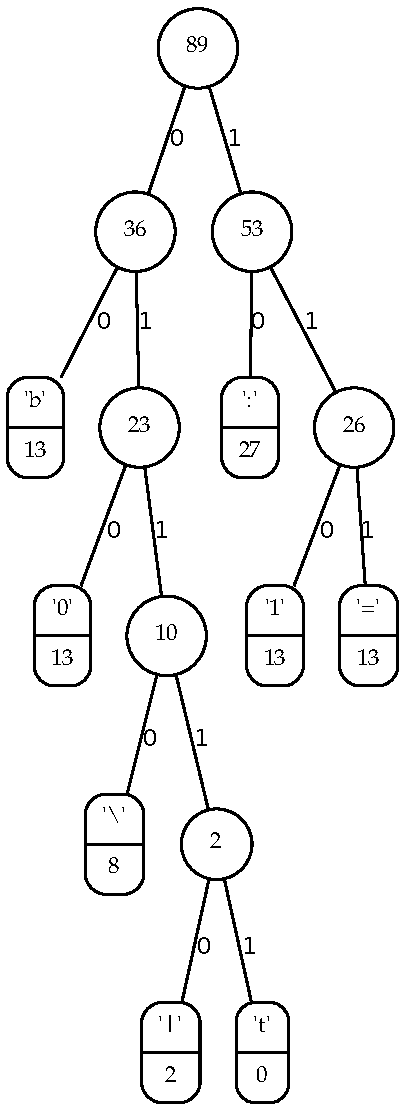
\includegraphics{optimizations/huffman.pdf}
  \caption{Huffman tree for frequencies in table
    \ref{tab:huffman_freq}, \textsf{(?:(?:(?:[a-zA-Z]+ ?)+[,.;:] ?)*..)*}}
  \label{fig:huffman2}
\end{figure}

\section{Experiments}
\subsection{Perls debug output}
\subsubsection{\texttt{regexmach.pl}}
\label{sec:regexmach.pl}
\lstinputlisting[language=Perl]{../kode/regexmach.pl}


\section{Optimization scripts}
\subsection*{Memory usage}
\subsubsection*{\texttt{memoryusage.pl}}
\label{sec:memoryusage.pl}
\lstinputlisting[language=Perl]{../kode/memoryusage.pl}

\subsection*{Runtimes}
\subsubsection*{\texttt{runtimes.pl}}
\label{sec:runtimes.pl}
\lstinputlisting[language=Perl]{../kode/runtimes.pl}

\subsection*{Profiling}
\subsubsection*{\texttt{profiling.pl}}
\label{sec:profiling.pl}
\lstinputlisting[language=Perl]{../kode/profiling.pl}


\section{Benchmark scripts}
\subsection*{\texttt{backtrackingworstcase.pl}}
\label{sec:backtrackingworstcase.pl}
\lstinputlisting[language=Perl]{../kode/backtrackingworstcase.pl}


\subsection*{\texttt{backtrackingworstcase\_mem.pl}}
\label{sec:backtrackingworstcase_mem.pl}
\lstinputlisting[language=Perl]{../kode/backtrackingworstcase_mem.pl}


\subsection*{\texttt{dfaworstcase.pl}}
\label{sec:dfaworstcase.pl}
\lstinputlisting[language=Perl]{../kode/dfaworstcase.pl}


\subsection*{\texttt{dfaworstcase\_mem.pl}}
\label{sec:dfaworstcase_mem.pl}
\lstinputlisting[language=Perl]{../kode/dfaworstcase_mem.pl}


\subsection*{\texttt{email.pl}}
\label{sec:email.pl}
\lstinputlisting[language=Perl]{../kode/email.pl}


\subsection*{\texttt{email\_mem.pl}}
\label{sec:email_mem.pl}
\lstinputlisting[language=Perl]{../kode/email_mem.pl}


\subsection*{\texttt{email\_mbvsize.pl}}
\label{sec:email_mbvsize.pl}
\lstinputlisting[language=Perl]{../kode/email_mbvsize.pl}


\subsection*{\texttt{number.pl}}
\label{sec:number.pl}
\lstinputlisting[language=Perl]{../kode/number.pl}


\subsection*{\texttt{number\_mem.pl}}
\label{sec:number_mem.pl}
\lstinputlisting[language=Perl]{../kode/number_mem.pl}


\subsection*{\texttt{number\_mbvsize.pl}}
\label{sec:number_mbvsize.pl}
\lstinputlisting[language=Perl]{../kode/number_mbvsize.pl}




